\documentclass[12pt, oneside]{article}
\usepackage[T1]{fontenc}
\usepackage[spanish, es-tabla, es-lcroman]{babel}
\usepackage[utf8]{inputenc}
\usepackage[document]{ragged2e}
\usepackage{tcolorbox}
\tcbuselibrary{theorems}
\usepackage{cancel}
\usepackage{amssymb}
\usepackage{amsmath}
\usepackage{mathrsfs}
\usepackage{wrapfig}
\usepackage{fancyhdr}
\usepackage{colortbl}
\usepackage{diagbox}
\usepackage{longtable}
\usepackage{graphicx}
\usepackage{subcaption}
\usepackage{xcolor}
\usepackage{tikz}
\usetikzlibrary{positioning}
\usepackage{multicol}
\usepackage{multirow}
\usepackage{lastpage}
\usepackage{pdfpages}
\usepackage{listings}
\usepackage{blindtext}
\usepackage{fontawesome}
\spanishdecimal{.}
\usepackage[explicit]{titlesec}
\usepackage[colorlinks=true, linkcolor=black, citecolor=black, urlcolor=blue]{hyperref}
\usepackage[a4paper, total={16cm, 24cm}]{geometry}
\pagestyle{fancy}
\lhead{Muñoz Nuñez Ian Emmanuel}
\rhead{Implementación de Visión Artificial}
\lfoot{Visión Robótica}
\rfoot{CUCEI}
\renewcommand{\headrulewidth}{1pt}
\renewcommand{\footrulewidth}{1pt}
\def\columnseprulecolor{\color{magenta}}

\setlength{\headheight}{14.49998pt}
\setlength{\columnseprule}{1pt}

\usepackage[firstpage=true]{background}
\backgroundsetup{
    scale=1.5,
    color=black,
    opacity=0.3,
    angle=0,
    firstpage=true,
    contents={
        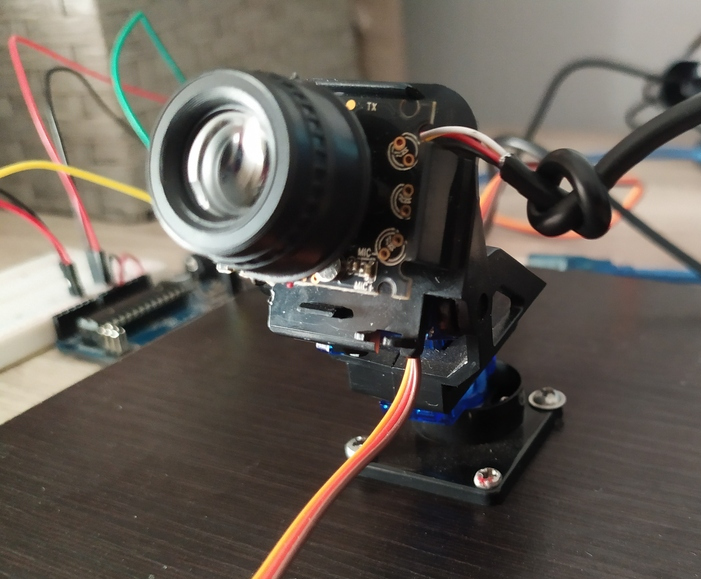
\includegraphics{back.jpg}
    }
}

\definecolor{basic}{RGB}{150, 150, 150}
\definecolor{fondo}{RGB}{40, 44, 51}
\definecolor{string}{RGB}{150, 50, 150}
\definecolor{keywords}{RGB}{0, 100, 150}
\definecolor{comment}{RGB}{0, 150, 50}

\lstdefinestyle{pythonScript}{
    language=python,
    basicstyle=\ttfamily\small\color{basic},
    backgroundcolor=\color{fondo},
    stringstyle=\color{string},
    commentstyle=\color{comment},
    emph={import, from, as, class, def, self, True, if, else, print, return, while, sum,
    raise, break, RuntimeError},
    emphstyle=\color{keywords},
    numbers=left,
    numberstyle=\ttfamily\scriptsize\color{black},
    numbersep=5pt,
    breakatwhitespace=true,
    breaklines=true,
    keepspaces=true,
    showspaces=false,
    showstringspaces=false,
    showtabs=false,
    xleftmargin=10pt,
    rulesepcolor=\color{magenta},
    frame=shadowbox
}
\lstdefinestyle{arduinoScript}{
    language=c,
    basicstyle=\ttfamily\small\color{basic},
    backgroundcolor=\color{fondo},
    stringstyle=\color{string},
    commentstyle=\color{comment},
    emph={if, else, print, return, while, void, int, setup, loop, delay, Serial,
    attach, read, write, available, include, Servo, begin},
    emphstyle=\color{keywords},
    numbers=left,
    numberstyle=\ttfamily\scriptsize\color{black},
    numbersep=5pt,
    breakatwhitespace=true,
    breaklines=true,
    keepspaces=true,
    showspaces=false,
    showstringspaces=false,
    showtabs=false,
    xleftmargin=10pt,
    rulesepcolor=\color{magenta},
    frame=shadowbox
}

\begin{document}

\begin{titlepage}
    \pagenumbering{roman}
    \centering
    {\bfseries\LARGE Universidad de Guadalajara \par}
    \vfill
    {
        
\includegraphics[width=0.3\linewidth]{UdG.png}
        
\includegraphics[width=0.3\linewidth]{qci.png}
        \par
    }
    \vfill
    {\bfseries\LARGE Proyecto \par}
    \vfill
    {\bfseries\LARGE Implementación de Visión Artificial \par}
    \vfill
    {\bfseries\LARGE Muñoz Nuñez Ian Emmanuel \par}
    \vfill
    {\bfseries\LARGE Visión Robótica \par}
\end{titlepage}

\pagenumbering{arabic}

\newpage
\section{Introducción}
{\sffamily\large\justify
    \hspace{0.5cm} En este proyecto se desarrollará el seguimiento de algún color usando
    técnicas, métodos y herramientas para el procesamiento de imágenes que nos ayuden a
    detectar el color deseado en la imagen. Para este proyecto se usaron servomotores
    \emph{SG90} controlados desde una tarjeta \emph{Arduino Uno}, y esta tiene una
    conexión serial con la computadora, la cuál recibe las imágenes de una cámara web
    externa.

    \hspace{0.5cm} Para desarrollar el proyecto se seleccionó el lenguaje de
    programación \emph{Python} pues se considero más ligero y rápido en comparación a
    \emph{MatLab}, además, \emph{Python} tiene muchas herramientas que nos ayudarán con
    el procesamiento de las imágenes obtenidas y con la conexión serial con la
    \emph{Arduino}, el procesamiento de las imágenes y la conexión serial son muy
    ligeras y rápidas, con lo que se obtuvo un comportamiento del sistema muy bueno.

}

\section{Objetivo}
{\sffamily\large\justify
    \hspace{0.5cm} En este proyecto se espera lograr tener un prototipo mínimamente
    funcional empleando una cámara web que se pueda sentar en una base con dos servos,
    estos servos se encargarán de corregir la orientación de la cámara para mantener el
    centroide de un objeto de color lo más en el centro posible de la imagen.

    \hspace{0.5cm} Las imágenes obtenidas por la cámara se usarán para aplicar filtros
    que pueden detectar un color, aunque también se aplicará ruido a estas imágenes y se
    usará otro filtro para tratar de minimizar ese ruido lo más posible, luego de
    realizar todo esto se tiene pensado obtener el centroide del objeto y calculando
    errores y ángulos enviar esta información por conexión serial.

    \hspace{0.5cm} En resumen, los objetivos que se desean son:
    \renewcommand{\labelitemi}{$\bullet$}
    \begin{itemize}
        \item Capturar imágenes de una cámara web externa que pueda moverse con los
            servos.
        \item Aplicar ruido mediante software a las imágenes obtenidas.
        \item Minimizar los más posible el ruido aplicado mediante un filtro.
        \item Detectar un color deseado.
        \item Obtener el centroide del objeto.
        \item Calcular el error del centroide y calcular los ángulos necesarios para
            corregir ese error.
        \item Realizar una comunicación serial con la \emph{Arduino Uno}.
    \end{itemize}

}

\newpage
\section{Desarrollo}
\subsection{Material utilizado}
{\sffamily\large\justify
    \begin{figure}[h!]
        \centering
        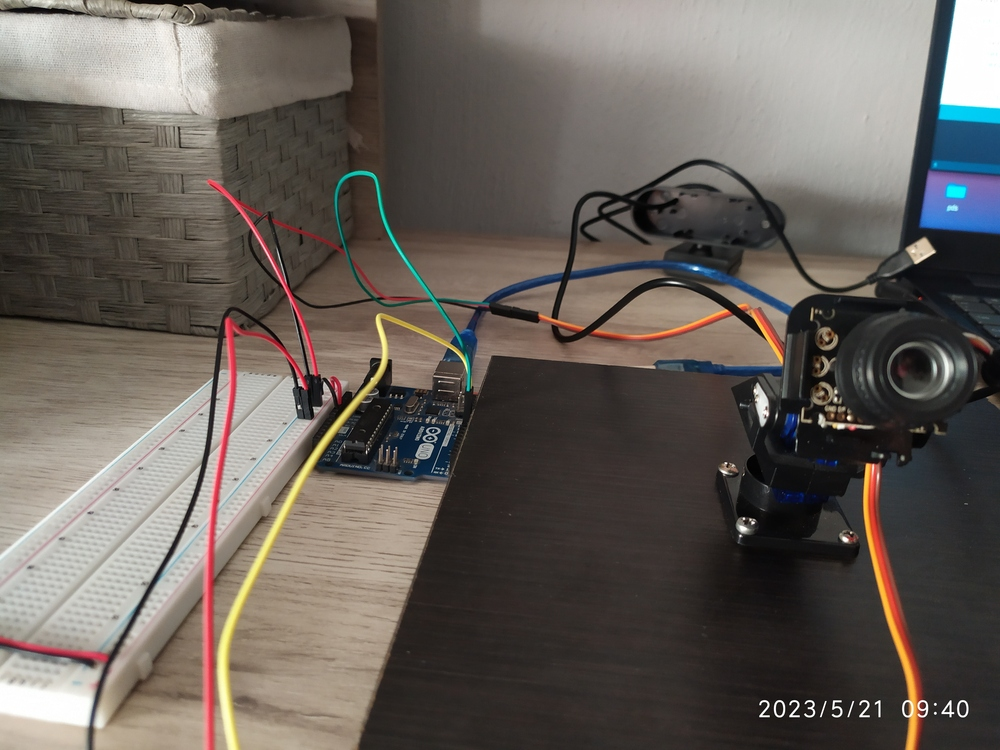
\includegraphics[width=0.8\linewidth]{figs/IMG_20230521_094011.jpg}
        \caption{\sffamily Foto del sistema terminado}
        \label{fig:elProyecto}
    \end{figure}

    \hspace{0.5cm} Para realizar el proyecto se usaron los siguientes componentes:
    \renewcommand{\labelitemi}{$\bullet$}
    \begin{itemize}
        \item Cámara web.
        \item Placa \emph{Arduino Uno}.
        \item 2 servomotores \emph{SG90}.
        \item Protoboard (para conectar los servos con la \emph{Arduino}).
    \end{itemize}

    \hspace{0.5cm} Otros materiales usados fueron:
    \begin{itemize}
        \item Base para 2 servomotores y cámara.
        \item Pandel de madera \emph{MDF} de \emph{16mm} de grosor.
        \item 4 tornillos (para perforar la madera).
    \end{itemize}

}

\newpage
\subsection{Primeros pasos}
{\sffamily\large\justify
    \hspace{0.5cm} El primer paso que se quería cumplir fue detectar el color en una
    imagen, y con esto poder calcular su centroide. Para esto se usó el siguiente
    código.

    \lstset{style=pythonScript}
    \begin{lstlisting}
while True:
    leido, video = captura.read() # Lectura de la camara
    video = cv2.resize(video, None, fx=0.4, fy=0.4) # Redimension del video
    m, n = video.shape[0:2] # Dimensiones del video

    hsv = cv2.cvtColor(video, cv2.COLOR_BGR2HSV) # Espacio de color de BGR a HSV
    mask = cv2.inRange(hsv, (15, 50, 50), (45, 255, 255)) # Mascara de color
    norm = cv2.normalize(mask.astype(float), None, 0.0, 1.0, cv2.NORM_MINMAX) # Normalizacion de 0 a 1
    norm = cv2.erode(norm, kernel) # Aplicacion de la erosion

    posy, posx = np.where(norm==1) # Posiciones de los 1's
    try:
        cy = int(np.sum(posy)/np.sum(norm)) # Posicion del centroide en 'y'
        cx = int(np.sum(posx)/np.sum(norm)) # Posicion del centroide en 'x'
    except:
        cy = int(m/2) # Posicion del centroide en 'y'
        cx = int(n/2) # Posicion del centroide en 'x'
        pass
    cv2.circle(video, (cx, cy), 5, (0, 255, 255), -1) # Circulo del centroide en el video

    if not leido: # Si hay un error con la lectura se termina el ciclo
        break

    if cv2.waitKey(1) == 27: # Si se presiona 'esc' se termain el ciclo
        break

    cv2.imshow("Video", video) # Se muestra el video
    cv2.imshow('Mask', norm) # Se muestra la mascara
    \end{lstlisting}

    \hspace{0.5cm} Para el procesamiento de imágenes se usó la librería \emph{opencv} de
    \emph{Python} y para algunos filtros y kernel's se uitlizó la librería \emph{numpy}.

    \hspace{0.5cm} El proyecto hasta este punto funcionó como se esperaba.

}

\newpage
\subsection{Obtención del error}
{\sffamily\large\justify
    \hspace{0.5cm} Para calcular el error de se usó la posición del centroide y las
    dimensiones de la imagen, esto para calcular el centro de esta, para calcular los
    error se usarón las fórmulas

    \begin{equation*}
        \begin{split}
            e_y & = \dfrac{m}{2} - c_y \\
            e_x & = \dfrac{n}{2} - c_x
        \end{split}
    \end{equation*}

    \hspace{0.5cm} Siendo $m$ y $n$ las filas y columnas de la imagen respectivamente,
    y siendo $c_y$ y $c_x$ la posición en $y$ y en $x$ del centroide.

    \hspace{0.5cm} En el código se agregaron las siguientes líneas.

    \lstset{style=pythonScript}
    \begin{lstlisting}
e_y = (m/2)-c_y
e_x = (n/2)-c_x
print(f'e_y: {e_y}')
print(f'e_x: {e_x}')
    \end{lstlisting}

    \hspace{0.5cm} En este punto, al igual que en el anterior todo funcionó
    correctamente.

}

\subsection{Conexión serial con la \emph{Arduino Uno}}
{\sffamily\large\justify
    \hspace{0.5cm} Luego de obtener el error, se probó la conexión con la
    \emph{Arduino Uno} y un solo servomotor. Para esto se agregaron algunas líneas más
    al código y se utilizó la librería \emph{pyserial}.

    \begin{lstlisting}[style=pythonScript]
uno = serial.Serial("/dev/ttyACM0", baudrate=9600, timeout=1)
    \end{lstlisting}

    \hspace{0.5cm} El código anterior funciona para crear una conexión serial con la
    tarjeta \emph{Arduino} desde \emph{Python}, también se agregaron las siguientes
    líneas

    \begin{lstlisting}[style=pythonScript]
angleX = chr(int(90+e_x))
uno.write(f"{angleX}".encode())
    \end{lstlisting}

    \hspace{0.5cm} En estas líneas se obtiene el ángulo que tiene que girar el servo
    para corregir el error obtenido. Para hacer esto, se observó que el ángulo de visión
    de la cámara usada era de aproximadamente 90°, de esta forma, se decidió dividir
    la imagen en 2, y dejar 45° de un lado y 45° de otro, y así, hacer que la
    configuración inicial del servo sea de 90°, con esto el servo se puede mover sin
    problemas y seguir el objeto, además, la imagen obtenida se redimensiona a 180
    pixeles, por lo que así es fácil calcular un ángulo, aunque en esta ocasión solo era
    una prueba, por lo que el ángulo puede tomar valores desde 0 hasta 180. Al final, la
    fórmula para calcular el ángulo resulta ser.

    \begin{equation*}
        \begin{split}
            angle_x & = 90^\circ + e_x \\
            angle_y & = 90^\circ + e_y
        \end{split}
    \end{equation*}

    \hspace{0.5cm} En este caso, no se necesitaron muchos cálculos, pues la imagen se
    adapto para que los errores solo fueran de \emph{-90°} hasta \emph{90°}, y al hacer
    una suma tan sencilla se puede calcular un ángulo. En este punto cada pixel
    representaría un grado de giro, más adelante se ajusta este detalle.

    \hspace{0.5cm} En esta parte del proyecto también se creo un código en
    \emph{Arduino} para la conexión serial.

    \begin{lstlisting}[style=arduinoScript]
#include <Servo.h>

Servo servoMotor;
int angle=90, in;

void setup()
{
    Serial.begin(9600);
    servoMotor.attach(9);
    servoMotor.write(angle);
    delay(100);
}

void loop()
{
    if(Serial.available() > 0)
    {
        in = Serial.read();
        servoMotor.write(angle);
    }
    angle = in;
}

    \end{lstlisting}

}

\newpage
\subsection{Conexión con servo \emph{x} y servo \emph{y}}
{\sffamily\large\justify
    \hspace{0.5cm} En este punto solo se agregó una línea de código

    \begin{lstlisting}[style=pythonScript]
uno.write(f"{angleY}".encode()) # Se envia el angulo 'y' Arduino
    \end{lstlisting}

    \hspace{0.5cm} El código en \emph{Arduino} fue el que resultó con más modificaciones

    \begin{lstlisting}[style=arduinoScript]
#include <Servo.h>

Servo servoX;
Servo servoY;
int inX, inY;
int angleX=90, angleY=90;

void setup()
{
    Serial.begin(9600);
    servoX.attach(9);
    servoY.attach(10);
    servoX.write(angleX);
    servoY.write(angleY);
    delay(100);
}

void loop()
{
    if(Serial.available() > 0)
    {
        inX = Serial.read();
        delay(50);
        inY = Serial.read();

        servoX.write(angleX);
        servoY.write(angleY);
    }
    angleX = inX;
    angleY = inY;
}
    \end{lstlisting}

}

\newpage
\subsection{Uso de la cámara externa y la base de servos}
{\sffamily\normalsize\justify
    \hspace{0.5cm} Al usar la cámara externa y la base con los servos, surgió un error
    con la implementación anterior, pues la manera de calcular el error y los ángulos
    no era la correcta, pues todo el tiempo de tuvo como referencia una cámara estática
    que, con el movimiento de los servos no se movía. Al tener la cámara en la base, el
    error se calculaba bien, pero al tratar de corregir el error con los servos, este
    influía al ángulo, por lo que mientras más se acercaba al error, menor se volvía el
    ángulo, algo obviamente ilógico, y al ocurrir esto, la la base y la cámara solo se
    movían de un lado a otro sin sentido, por lo que se usó una idea distinta para todo
    esto. Con esta idea, los códigos terminaron de la siguiente manera

    \begin{lstlisting}[style=pythonScript]
import cv2 as cv
import numpy as np
import serial
from time import sleep

captura = cv.VideoCapture(2) # Conexion con la camara 0/2

kernel = np.ones((9, 9), dtype=np.uint8) # Kernel para la erosion

uno = serial.Serial("/dev/ttyACM0", 9600, write_timeout=10) # Conexion serial con Arduino
sleep(2) # Espera de 2 segundos para realizar la conexion serial correctamente

angleY = chr(90) # Inicializacion del angulo en 'y' en 90 grados
angleX = chr(90) # Inicializacion del angulo en 'x' en 90 grados
minAngle = 45 # Angulo minimo al que deben girar los motores
maxAngle = 135 # Angulo maximo al que deben girar los motores

while True:
    leido, video = captura.read() # Lectura de la camara
    video = cv.resize(video, (180, 180)) # Redimension del video
    video = cv.flip(video, 0) # Voltear el video en el eje 'x'
    m, n = video.shape[0:2] # Dimensiones del video

    hsv = cv.cvtColor(video, cv.COLOR_BGR2HSV) # Espacio de color de BGR a HSV
    mask = cv.inRange(hsv, (50, 0, 0), (80, 255, 255)) # Mascara de color rosa
    norm = cv.normalize(mask.astype(float), None, 0.0, 1.0, cv.NORM_MINMAX) # Normalizacion de 0 a 1
    norm = cv.erode(norm, kernel) # Aplicacion de la erosion

    posy, posx = np.where(norm==1) # Posiciones de los 1's
    try:
        cy = int(np.sum(posy)/np.sum(norm)) # Posicion del centroide en 'y'
        cx = int(np.sum(posx)/np.sum(norm)) # Posicion del centroide en 'x'
    except:
        cy = int(m/2) # Posicion del centroide en 'y'
        cx = int(n/2) # Posicion del centroide en 'x'
    cv.circle(video, (cx, cy), 5, (0, 255, 0), -1) # Circulo del centroide en el video

    e_y = -((m/2)-cy) # Error en 'y'
    e_x = -((n/2)-cx) # Error en 'x'

    if abs(e_y) > 10: # Si el error de 'y' es mayor a 10
        angleY = ord(angleY) # Convertir 'angleY' de chr a int
        angleY = angleY + int(e_y*0.05) # Accion de control para el angulo en 'y'
        angleY = max(minAngle, angleY) # Cota minima del angulo en 'y'
        angleY = min(maxAngle, angleY) # Cota maxima del angulo en 'y'
        angleY = chr(angleY) # Convertir 'angleY' de int a chr

    if abs(e_x) > 10: # Si el error de 'x' es mayor a 10
        angleX = ord(angleX) # Convertir 'angleX' de chr a int
        angleX = angleX + int(e_x*0.05) # Accion de control
        angleX = max(minAngle, angleX) # Cota minima del angulo en 'x'
        angleX = min(maxAngle, angleX) # Cota maxima del angulo en 'x'
        angleX = chr(angleX) # Convertir 'angleX' de int a chr

    uno.write(f"{angleX}".encode()) # Se envia el angulo 'x' Arduino
    uno.write(f"{angleY}".encode()) # Se envia el angulo 'y' Arduino

    if not leido: # Si hay un error con la lectura se termina el ciclo
        break

    if cv.waitKey(1) == 27: # Si se presiona 'esc' se termain el ciclo
        break

    cv.imshow("Video", video) # Se muestra el video
    cv.imshow('Mask', norm) # Se muestra la mascara

uno.close() # Cierre de la conexion serial con la Arduino Uno
captura.release() # Se libera la captura
cv.destroyAllWindows() # Se cierran todas las ventanas
    \end{lstlisting}

    \newpage
    \hspace{0.5cm} El código en \emph{Python} resultó con muchas diferencias en
    comparación a los códigos anteriores. Pues se agregarón muchas otras operaciones y
    funciones al código.

    \hspace{0.5cm} El código en \emph{Arduino} no cambio mucho

    \begin{lstlisting}[style=arduinoScript]
#include <Servo.h>

Servo servoX; // Servo para el eje 'x'
Servo servoY; // Servo para el eje 'y'
int inX, inY; // Variables para recibir datos desde Python
int angleX=90, angleY=90; // Variables para enviar angulos a los servos

void setup()
{
    Serial.begin(9600); // Comunicacion serial con 9600 baudios
    Serial.setTimeout(10); // Espera de 10 milisegundos entre cada lectura

    servoX.attach(9); // Asignar pin 9 para el servo del eje 'x'
    servoY.attach(10); // Asignar pin 10 para el servo del eje 'y'

    servoX.write(angleX); // Se mueve el servo del eje 'x' a 90 grados
    servoY.write(angleY); // Se muevo el servo del eje 'y' a 90 grados

    delay(100); // Espera de 100 milisegundos (0.1 segundos)
}

void loop()
{
    if(Serial.available() > 0) // Si la comunicacion serial esta en uso
    {
        inX = Serial.read(); // Recibir el angulo para el servo del eje 'x'
        delay(10); // Espera de 10 milisegundos (0.01 segundos)
        inY = Serial.read(); // Recibir el angulo para el servo del eje 'y'

        servoX.write(angleX); // Se envia el valor 'angleX' al servo del eje 'x'
        servoY.write(angleY); // Se envia el valor 'angleY' al servo del eje 'y'
    }

    angleX = inX; // El angulo en 'x' es igual al valor 'x' recibido
    angleY = inY; // El angulo en 'y' es igual al valor 'y' recibido
}
    \end{lstlisting}

    \hspace{0.5cm} En este punto ya se tenía un prototipo funcional, aunque aún hacia
    falta agregarle ruido artificial a la imagen y aplicar un filtro para minimizarlo.

}

\subsection{Ruido y aplicación del filtro}
{\sffamily\large\justify
    \hspace{0.5cm} Por último, se agregó el ruido a la imagen con las siguientes líneas

    \begin{lstlisting}[style=pythonScript]
noiseMatrix = np.random.normal(-0.5, 0.5, video.size)
gaussNoise = noiseMatrix.reshape(video.shape[0], video.shape[1], video.shape[2]).astype('uint8')
videoNoise = cv.add(video, gaussNoise)
    \end{lstlisting}

    \hspace{0.5cm} Para aplicar un filtro de difuminado se usaron estas líneas

    \begin{lstlisting}[style=pythonScript]
f = np.ones((11, 11), dtype=np.float32)*1/121
videoFiltro = cv.filter2D(videoNoise, -1, f)
    \end{lstlisting}

    \hspace{0.5cm} Con estas líneas, se logró hacer que el color fuera lo
    suficientemente claro para que el algoritmo lo detectara y el programa siga
    funcionando como antes.

}

\newpage
\section{Resultados}
\subsection{Prototipo}
{\sffamily\large\justify
    \begin{figure}[h!]
        \centering

        \begin{subfigure}[tl]{0.45\textwidth}
            \centering
            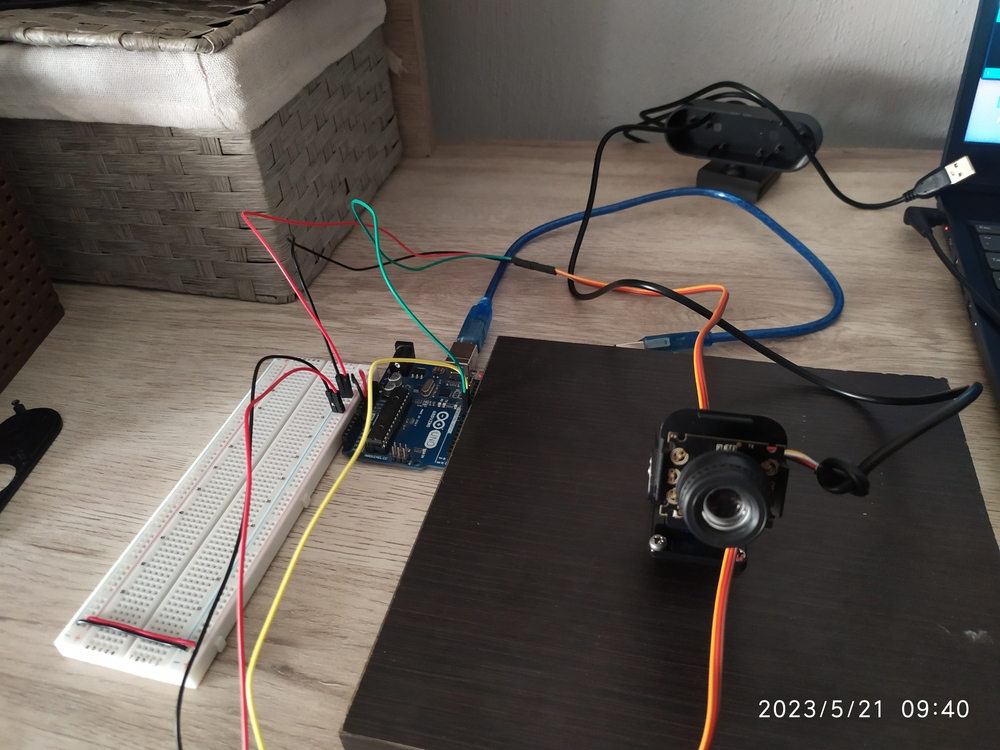
\includegraphics[width=\linewidth]{figs/IMG_20230521_094003.jpg}
        \end{subfigure}
        \begin{subfigure}[tr]{0.45\textwidth}
            \centering
            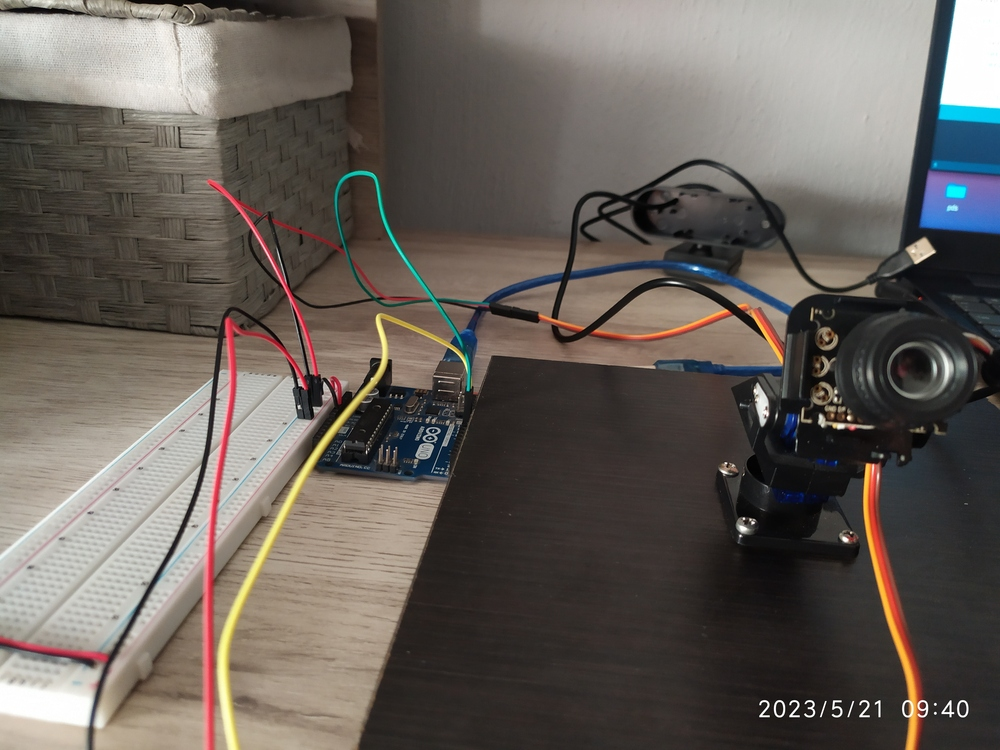
\includegraphics[width=\linewidth]{figs/IMG_20230521_094011.jpg}
        \end{subfigure}
        \begin{subfigure}[bl]{0.45\textwidth}
            \centering
            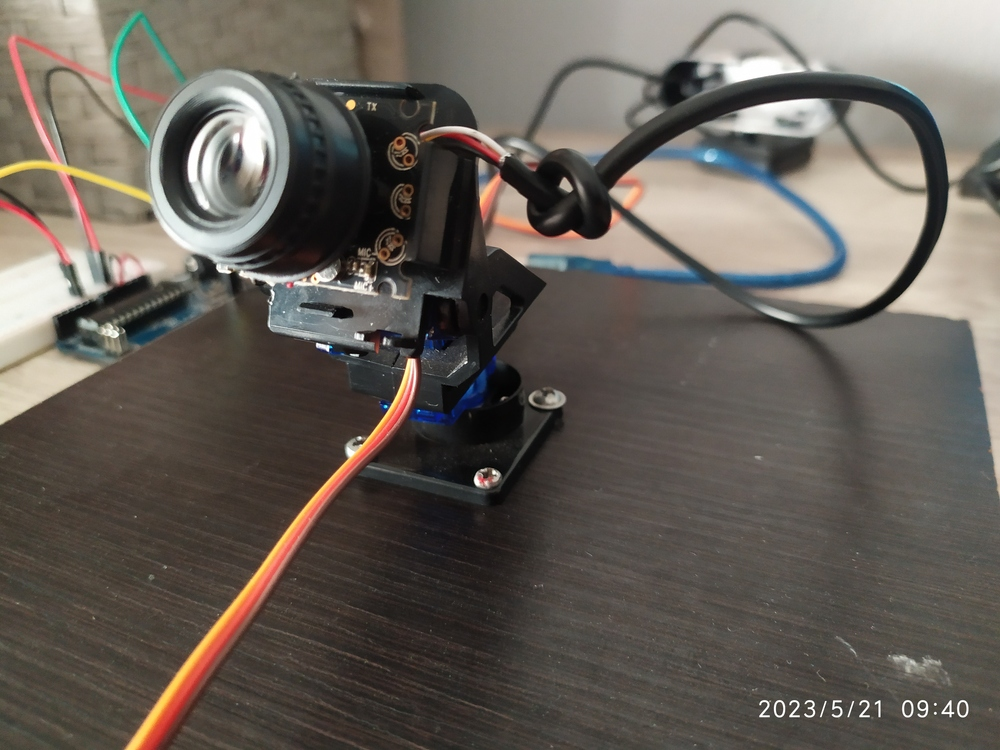
\includegraphics[width=\linewidth]{figs/IMG_20230521_094025.jpg}
        \end{subfigure}
        \begin{subfigure}[br]{0.45\textwidth}
            \centering
            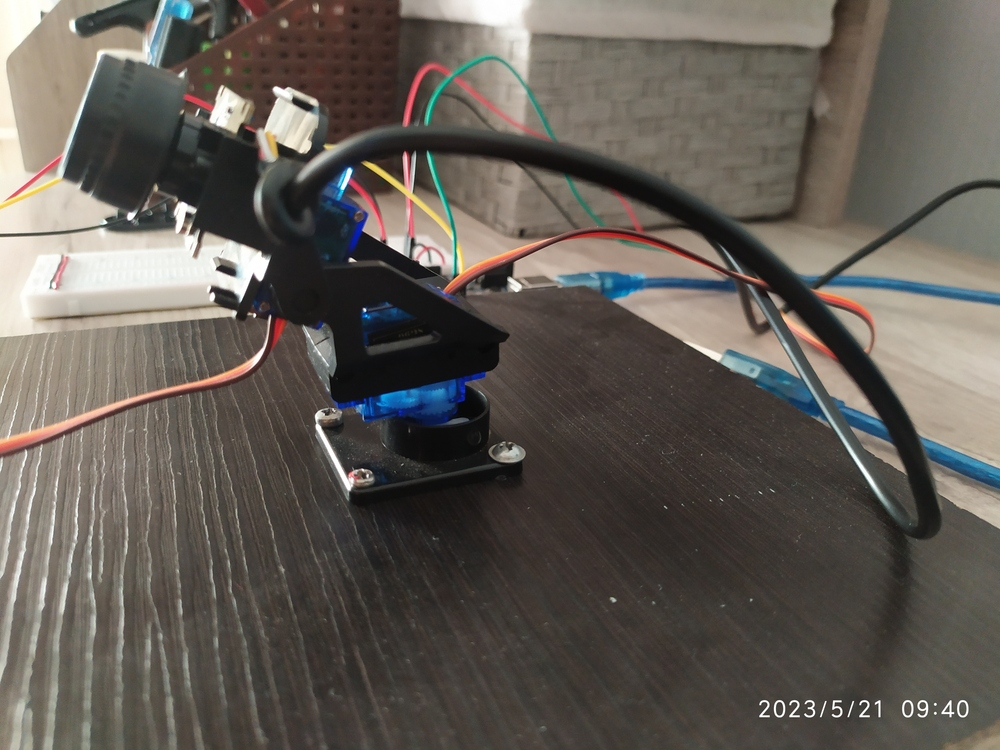
\includegraphics[width=\linewidth]{figs/IMG_20230521_094036.jpg}
        \end{subfigure}

        \caption{\sffamily Prototipo terminado}
        \label{fig:prototipo}
    \end{figure}

    \hspace{0.5cm} El prototipo terminado se puede observar en las imágenes de arriba,
    se puede observar que la base se atornillo a un panel de madera \emph{MDF} para que
    no se caiga con los movimientos de los servos y el peso de la cámara, el panel tiene
    una medida de \emph{200mm x 200mm x 16mm}, ya que el panel media más, se corto para
    que fuera más pequeño y un poco más ligero, esto para que no sea pesado al cargarlo
    en una mochila.

}

\newpage
\subsection{Imágenes de entrada y salida}
{\sffamily\large\justify
    \begin{figure}[h!]
        \centering

        \begin{subfigure}[tl]{0.35\textwidth}
            \centering
            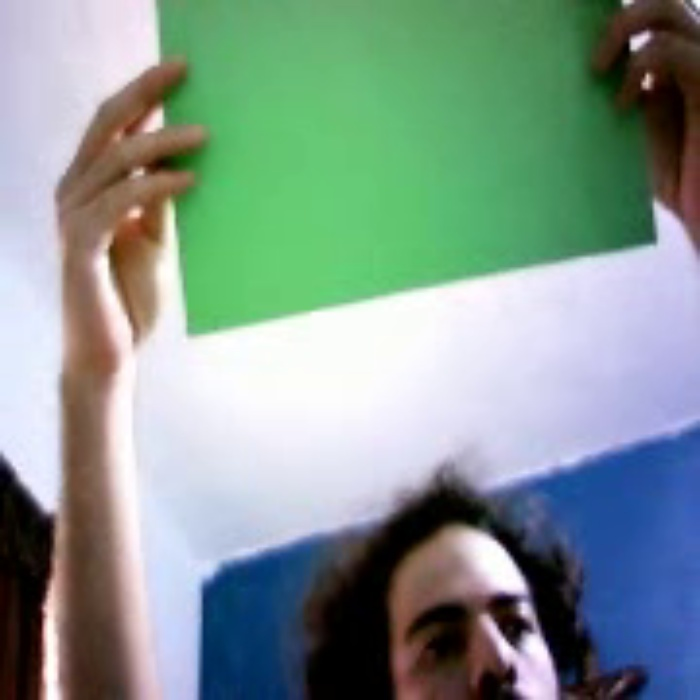
\includegraphics[width=\linewidth]{video.jpg}
            \caption{\sffamily Video de entrada}
        \end{subfigure}
        \begin{subfigure}[tr]{0.35\textwidth}
            \centering
            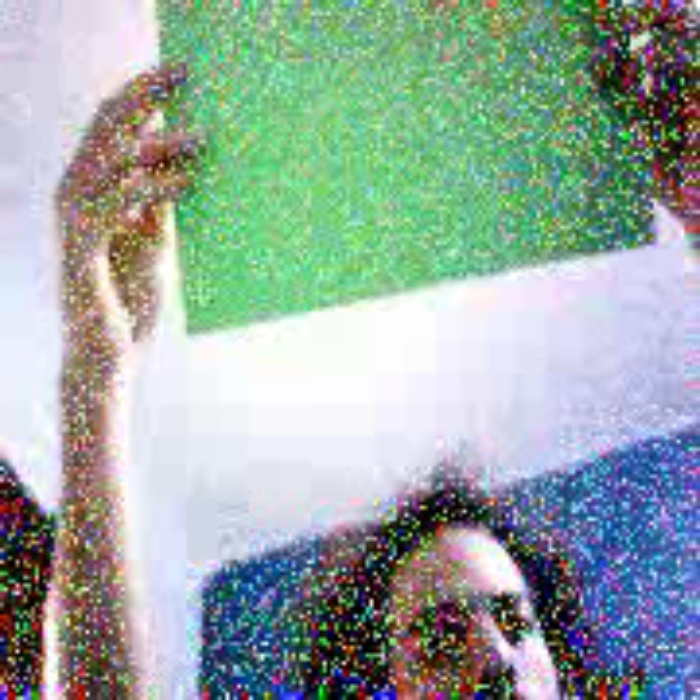
\includegraphics[width=\linewidth]{noise.jpg}
            \caption{\sffamily Ruido aplicado al video}
        \end{subfigure}
        \begin{subfigure}[bl]{0.35\textwidth}
            \centering
            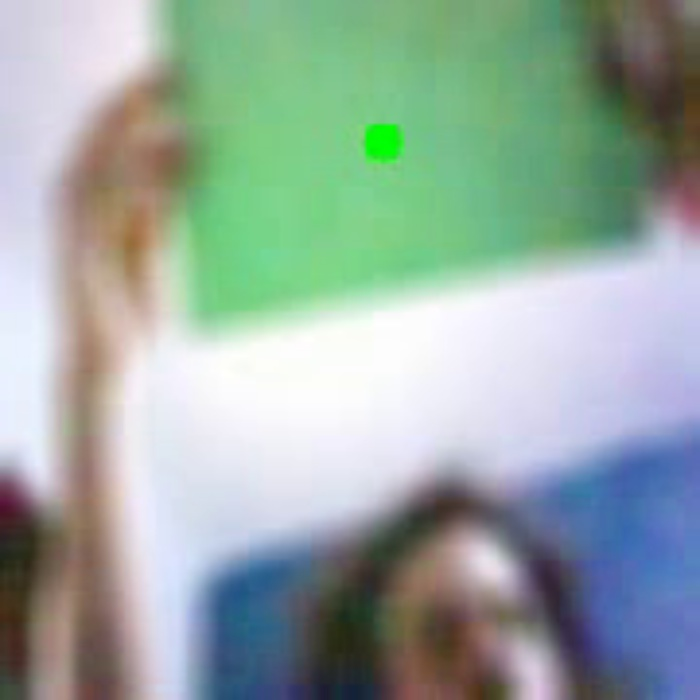
\includegraphics[width=\linewidth]{filter.jpg}
            \caption{\sffamily Video con el ruido filtrado}
        \end{subfigure}
        \begin{subfigure}[br]{0.35\textwidth}
            \centering
            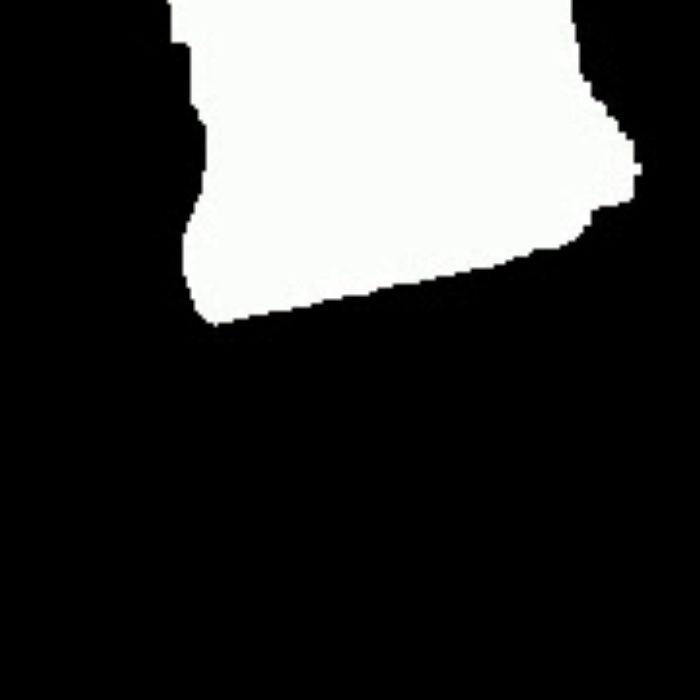
\includegraphics[width=\linewidth]{mask.jpg}
            \caption{\sffamily Máscara aplicada al video filtrado}
        \end{subfigure}

        \caption{\sffamily Imágenes de entrada y salida}
        \label{fig:imagenes}
    \end{figure}

    \hspace{0.5cm} En la imagen de la esquina superior izquierda se muestra la imagen
    obtenida de la cámara, al lado se muestra la imagen resultante con el ruido
    aplicado, la de la esquina inferior izquierda muestra la imagen con el filtro
    aplicado para minimizar el ruido, y por último, aparece la máscara aplicada a la
    imagen con el filtro para el ruido, esta última se uso para calcular el centroide
    del objeto y con esto obtener errores y valores de ángulos.

}

\newpage
\subsection{Gráficas}
{\sffamily\large\justify
    \begin{figure}[h!]
        \centering

        \begin{subfigure}{0.4\textwidth}
            \centering
            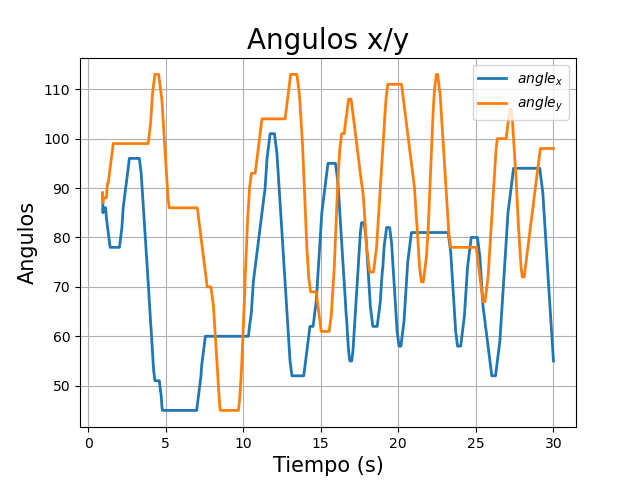
\includegraphics[width=\linewidth]{angulos.png}
            \caption{\sffamily Ángulos}
        \end{subfigure}
        \begin{subfigure}{0.4\textwidth}
            \centering
            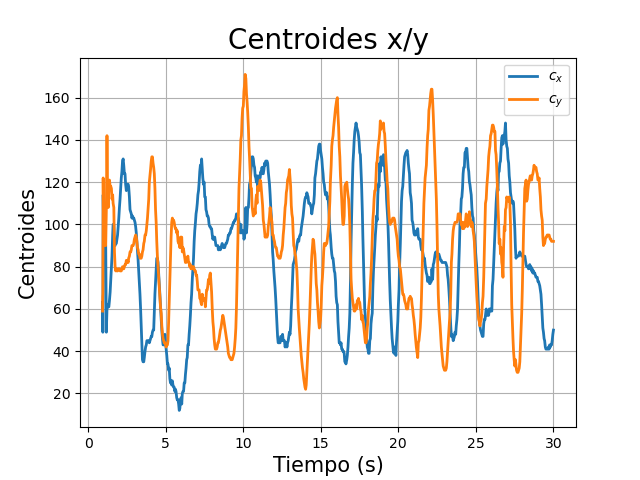
\includegraphics[width=\linewidth]{centroide.png}
            \caption{\sffamily Centroide}
        \end{subfigure}
        \begin{subfigure}{0.4\textwidth}
            \centering
            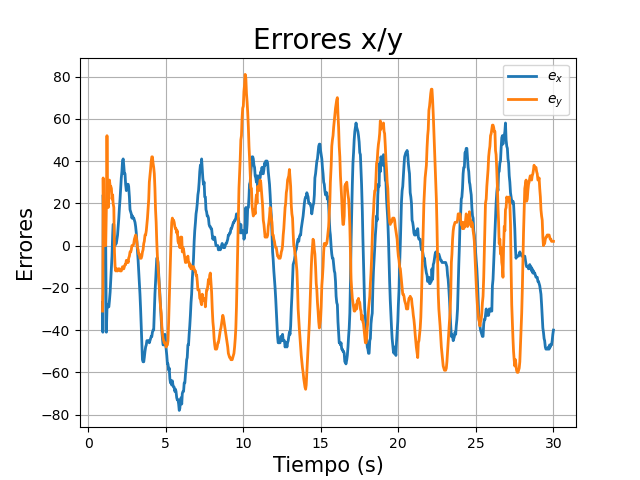
\includegraphics[width=\linewidth]{error.png}
            \caption{\sffamily Error}
        \end{subfigure}

        \caption{\sffamily Gráficas}
        \label{fig:graficas}
    \end{figure}

    \hspace{0.5cm} Para tomar valores y errores del proyecto, se corrieron los programas
    por 30 segundos, las gráficas muestran los valores de los ángulos de los servos, la
    posición del centroide y el error del centroide respecto al centro de la imagen
    durante estos 30 segundos.

    \hspace{0.5cm} Se puede ver que la gráfica del centroide y del error es muy
    parecida, esto es porque están directamente relacionados, solo que el centroide se
    mueve al rededor de los 90°, pues los 90° fueron tomados como el ángulo central de
    la imagen, en cambio, el error se mueve al rededor del $0$, pues esta gráfica
    muestra cuan lejos estaba el centroide del objeto del centro de la imagen.

}

\newpage
\section{Conclusiones}
{\sffamily\large\justify
    \hspace{0.5cm} Este proyecto fue muy interesante, pues desarrollarlo y lograr hacer
    que cada objetivo deseado se cumpliera y funcionara correctamente fue difícil, pero
    es gratificante observar como cada objetivo se va cumpliendo y ver como al final, el
    proyecto funciona correctamente.

    \hspace{0.5cm} Tal vez lo más complicado fue lograr que la conexión serial con la
    \emph{Arduino} funcionara correctamente, además, fue complicado desarrollar una idea
    completamente nueva en medio del desarrollo del proyecto para solucionar el problema
    de los ángulos para los servos.

    \hspace{0.5cm} A pesar de solo haber usado un controlador proporcional, el
    comportamiento y la corrección del error fueron muy buenos, aunque usando un control
    \emph{PID} se podría tener un mejor resultado, pero lamentablemente no se tuvo el
    tiempo suficiente para poder implementarlo y mejorarlo.

    \hspace{0.5cm} Considero que este proyecto se podría adaptar muy fácil a sistemas de
    vigilancia y seguimiento de objetos, no solamente de objetos de color, aunque le
    hacen falta algunas mejoras.

}

\end{document}

